
\documentclass[11pt,a4paper]{article}
\author{TalentSprint}
\date{}
\usepackage{verbatim}
\usepackage{fancyhdr}           % For header and footer
\usepackage{multicol}
\usepackage{colortbl}           % For coloured tables
\usepackage{setspace}           % For line height
\usepackage{seqsplit}           % Splits long words.
\usepackage{amsmath} 
\usepackage{graphicx}
\usepackage{array}
\usepackage{enumitem}
\usepackage{xcolor}
\usepackage[tikz]{bclogo}
\usepackage{textcomp}
\usepackage{listings}
\lstset{language=python,numbers=left,numberstyle=\tiny,numbersep=10pt,showstringspaces=false}

\headheight=14pt
\lhead{\nouppercase{}}
\rhead{\nouppercase{\leftmark}}

\newcommand*\lstinputpath[1]{\lstset{inputpath=#1}}
\lstinputpath{../Code/}
\graphicspath{{../Images/} {../ScreenShots/}}

\setcounter{tocdepth}{1}
\setlength\parindent{0pt}
\parskip=4pt
\newcommand{\Code}[1]{\textbf{\texttt{#1}}}

% Lengths and widths
\addtolength{\textwidth}{5cm}
\addtolength{\hoffset}{-1cm}
\setlength{\headsep}{-12pt} % Reduce space between header and content
\setlength{\headheight}{85pt} % If less, LaTeX automatically increases it
\renewcommand{\footrulewidth}{2pt} % Remove footer line
\renewcommand{\headrulewidth}{1pt} % Remove header line
\renewcommand{\seqinsert}{\ifmmode\allowbreak\else\-\fi} % Hyphens in seqsplit
% This two commands together give roughly
% the right line height in the tables
\renewcommand{\arraystretch}{1.3}
\onehalfspacing

% Commands
\newcommand{\SetRowColor}[1]{\noalign{\gdef\RowColorName{#1}}\rowcolor{\RowColorName}} % Shortcut for row colour
\newcommand{\mymulticolumn}[3]{\multicolumn{#1}{>{\columncolor{white}}#2}{#3}} % For coloured multi-cols
\newcolumntype{x}[1]{>{\raggedright}p{#1}} % New column types for ragged-right paragraph columns
\newcommand{\tn}{\tabularnewline} % Required as custom column type in use

% Font and Colours
\definecolor{HeadBackground}{HTML}{333333}
\definecolor{FootBackground}{HTML}{666666}
\definecolor{TextColor}{HTML}{333333}
\definecolor{DarkBackground}{HTML}{6B8E23} %{FD1AA8}
\definecolor{LightBackground}{HTML}{E8FED8} %D3FDC8
\definecolor{tit}{HTML}{FF6600}
\renewcommand{\familydefault}{\sfdefault}
\color{TextColor}
 \headsep = 25pt
% Header and Footer
\pagestyle{fancy}
\usepackage[headheight=110pt]{geometry}
\fancyhf{}% Clear header/footer

\fancyhead[r]{
\includegraphics[width = 4cm, height = 2cm]{TS-Logo.png}\hspace{0cm}}

%=================================TITLE=====================================
\fancyhead[l]{\Large{\bf{\textcolor{tit}{\textrm{Pointers}}}}}
%===========================================================================

\renewcommand{\headrulewidth}{0.4pt}% Default \headrulewidth is 0.4pt
\renewcommand{\footrulewidth}{0.4pt}% Default \footrulewidth is 0pt

\rfoot{Page \thepage}
\lfoot{COPYRIGHT \textcopyright TALENTSPRINT, 2015. ALL RIGHTS RESERVED.}




\begin{document}

\section*{Pointers}
Pointers are variables that hold address of other variables.

Pointers are one of the most distinct and exciting features of C language. They provide power and flexibility.

\subsection*{Benefit of using pointers}
\begin{itemize}
\item Pointers are more efficient in handling Arrays and Strings.
\item Pointers allow passing of function as argument to other functions.
\item Pointer code is usually shorter and more efficient.
\item Pointers enable dynamic memory management.
\end{itemize}

\subsection*{Concept of Pointer}
Whenever a variable is declared, system will allocate a location to that variable in memory, to hold its value. The location where it is stored has a unique address.

Let us say that system has allocated memory location 80F for variable \textbf{\texttt{a}}.

\lstinline!int a = 10 ;!

\begin{figure}[ht]

\begin{center}
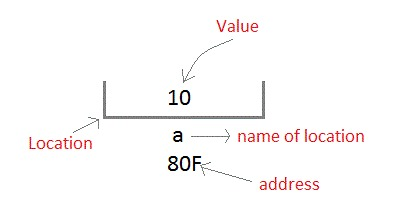
\includegraphics[scale=0.6]{variable_storage_in_c.jpg}
\caption{Variable Storage in C}
\label{var:storage}
\end{center}
\end{figure}

We can access the value 10 by either using the variable name \texttt{a} or the address 80F. Since the memory addresses are simply numbers, they can be assigned to some other variable. Variables that holds memory addresses are called \textbf{pointers}. A pointer variable is therefore nothing but a variable that contains an address, which is a location of another variable. 

\begin{figure}[ht]
\begin{center}
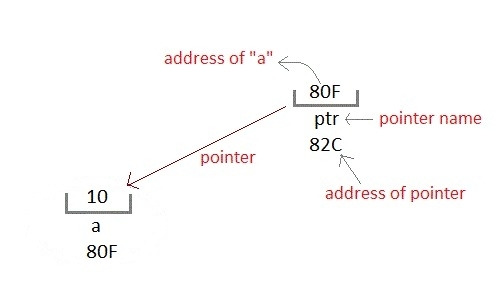
\includegraphics[scale=0.8]{pointer_to_variable.jpg}
\caption{Pointer to Variable}
\label{Pointer}
\end{center}
\end{figure}

\subsubsection*{Declaration} 
General syntax of pointer declaration is:

\textbf{\texttt{data-type* pointer-var;}}

Data type of pointer must be same as the variable, which the pointer is pointing. \lstinline!void! type pointer works with all data types, but isn't used often.

\subsubsection*{Initialization}
Pointer Initialization is the process of assigning a \emph{valid} address to a pointer variable.  The address operator `\textbf{\&}' is used to determine the address of a variable. The \& (immediately preceding a variable name) returns the address of the variable associated with it.

\begin{lstlisting}[numbers=none]
  int a = 10;
  int* ptr;  //pointer declaration
  ptr = &a;  //pointer initialization
\end{lstlisting}

    or as in, \lstinline!int* ptr = &a;! we can do initialization and declaration together.

\emph{A pointer variable should be initialized with the address of a variable of the same datatype. Otherwise there will be unpredictable program behaviour.}

\begin{lstlisting}[numbers=none]
    float a;
    int* ptr;
    ptr = &a;   //ERROR, type mismatch
\end{lstlisting}

\subsection*{Dereferencing}
Once a pointer has been assigned the address of a variable. To access the value of variable, pointer is \emph{dereferenced}, using the indirection operator \textbf{\texttt{`*'}}.

\begin{lstlisting}
#include <stdio.h>
int main() {
    int a;
    int* p;
    a = 10;
    p = &a;   
    printf("%d", *p);    //this will print the value of a. 
    printf("%d", *&a);   //this will also print the value of a.
    printf("%u", &a);    //this will print the address of a.
    printf("%u", p);     //this will also print the address of a.
    printf("%u", &p);    //this will also print the address of p.
    return 0;
}
\end{lstlisting}

\subsubsection*{Example}
Program to demonstrate pointer.

\lstinputlisting{Program-10-3.c}

\begin{figure}[ht]
\begin{center}
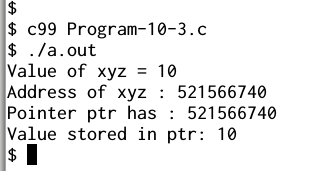
\includegraphics[scale=0.6]{Output-10-3.png}
\caption{Pointers and Addresses}
\label{output-10-3}
\end{center}
\end{figure}

\section*{Call Mechanisms}
There are two ways that arguments can be passed to a function:
\begin{itemize}
\item Call by Value
\item Call by Reference
\end{itemize}

By default, C uses call by value to pass arguments. In general, this means that code within a function cannot alter the arguments used to call the function. Whatever changes made to the values of the arguments are lost when the control exits the function.

\section*{Call by Value}
The \emph{call by value} method of passing arguments to a function copies the actual value of an argument into the formal parameter of the function. Because of this, changes made to the parameter inside the function have no effect on the argument.

The parameter in the called function is initialized with the value of the passed parameter. As long as the parameter has not been declared as constant, the value of the parameter can be changed; but the changes are relevant only within the scope of the called function. They have no effect on the value of the variable in the calling function.

See Figure \ref{output-10-4} for understanding the working of the code below:
 
\subsubsection*{Example}
 
\lstinputlisting{Program-10-4.c}

\begin{figure}[ht]
\begin{center}
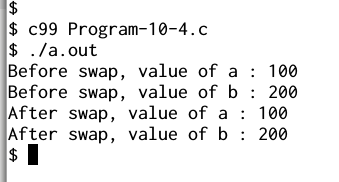
\includegraphics[scale=0.6]{Output-10-4.png}
\caption{Call by Value Swap}
\label{output-10-4}
\end{center}
\end{figure}

\section*{Call by Reference}
The \emph{call by reference} method of passing arguments to a function copies the address of an argument into the formal parameter. Inside the function, the address is used to access the actual argument used in the call. This means that changes made to the parameter affect the passed argument.

To pass by reference, argument pointers are passed to the functions just like any other value. So accordingly you need to declare the function parameters as pointer types.

\subsubsection*{Example}

\lstinputlisting{Program-10-5.c}

The function swap() is called, the actual values of the varaiables a and b are exchanged because they are passed by reference.

\begin{figure}[ht]
\begin{center}
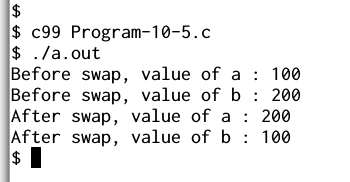
\includegraphics[scale=0.6]{Output-10-5.png}
\caption{Call by Reference Swap}
\label{output-10-5}
\end{center}
\end{figure}
\end{document}